In questa sottosezione ci occuperemo di descrivere nel dettaglio le equazioni
facenti capo a ciascun blocco funzionale precedentemente descritto:
%###
\paragraph{ Generatore dei riferimenti - Guidance:}
La funzione di questo blocco è quella di ricostruire il quaternione di
riferimento associato al riferimento LORF (Espresso nel sistema di riferimento
J2000) a partire dalle misure ricavate dall'unità GPS ($y_r$ posizione, $y_v$
velocità), richichiamando la definizione del LORF segue che:
\begin{equation}
	\mathfrak{R_0} = \{C,\bar{o}_1,\bar{o}_2,\bar{o}_3\}
\end{equation}

\begin{equation}
\bar{o}_1 = \frac{\vec{v}}{|\vec{v}|} \hspace{20pt}%
\bar{o}_2 = \frac{\vec{h}=\vec{r} \times \vec{v}}{|\vec{h}|} \hspace{20pt}%
\bar{o}_3 = \frac{\vec{e}=\bar{o}_1 \times \bar{o}_2}{|\vec{e}|}
\end{equation}

\begin{equation}
	\components{y_r}(t) = \components{r}(t) + \delta \components{r}(t)
\end{equation}

\begin{equation}
	\components{y_v}(t) = \components{v}(t) + \delta \components{v}(t)
\end{equation}

La matrice d'assetto LORF può essere ricavata come:
\begin{equation}
\underline{R_{0}^{i}}=
\begin{bmatrix}
	\frac{\components{y_v}}{|\components{y_v}|} &
	\frac{\components{y_h}=\components{y_r}	\times \components{y_v}}{|\components{y_h}|} &
	\frac{\components{y_e}=\components{y_v} \times (\components{y_r}\times\components{y_v})}{|\components{y_v}|}(t))
\end{bmatrix}
\end{equation}

La misura proventiente dal GPS é però affetta da errore per tanto definiamo la
matrice tenendo conto di una rotazione infinitesima definita
tramite gli angoli di eulero $\delta\components{\theta_0}$:
\begin{equation}
R_{0}^{i}=\underline{R_{0}^{i}}(I+\delta R_{0}^{i})
\end{equation}
\begin{equation}
\delta R_{0}^{i} = \delta\components{\theta_0} \times
\end{equation}
Un approssimazione degli angoli di eulero associati all'errore si ottiene
tramite la seguente relazione:

\begin{equation}
	\delta \boldsymbol{\theta_0}= \frac{1}{r}
	\begin{bmatrix}
	-\delta\vec{r}\cdot\vec{o}_2\\
	\delta\vec{r}\cdot\vec{o}_1-\frac{-\delta\vec{v}\cdot\vec{o}_3}{\omega_0}\\
	\frac{-\delta\vec{v}\cdot\vec{o}_2}{\omega_0}\\
	\end{bmatrix}
,\hspace{10pt} v\approx\omega_0 r 
\end{equation}

Calcoliamo adesso la varianza dell'errore di rotazione maggiorandola con una
quantità $\sigma^2_{0,max}$:
\begin{equation}
\xi[\delta\components{\theta_0}
\delta\components{\theta_0}^T]\le I \sigma^2_{0,max}
\end{equation}

Allocando la stessa varianza sia alla componente di posizione che di velocità
otteniamo che:

\begin{equation}
\sigma_r < \frac{(R_E + h)\cdot\sigma_{0,max}}{\sqrt{2}}
\end{equation}

\begin{equation}
\sigma_v < \frac{\omega_0\cdot r\cdot \sigma_{0,max}}{\sqrt{2}}
\end{equation}

tramite queste relazioni è possibile scegliere il sensore in grado di garantire
un errore angolare accettabile a partire dalle sue specifiche (varianza in
posizione e velocità).

Usando la conversione da matrice di assetto a quaternione è possibile calcolare
il quaternione di riferimento

\begin{equation}
	\underline{\components{\mathit{y_0}}}(t)=\underline{\components{\mathit{y_0}}}(\underline{R_{0}^{i}}(t))
\end{equation}

Svantaggio di questo approccio è l'impossibilità dell'ottenere il valore vero di
$\underline{R_{0}^{i}}$ poichè sarà sempre sporcato dall'errore di misura,
aggiungiamo quindi un predittore dello stato che ci permetta di filtrare questi
errori e che ci faccia guadagnare contemporaneamente anche la possibilità di
predirre il vettore accelerazione angolare orbitale
$\components{\underline{\dot{\omega}}}$ e velocità angolare orbitale
$\components{\underline{\omega}}$.
Definito l'incremento angolare come:
\begin{equation}
\components{\underline{\omega}^*} =\components{\underline{\omega}} \cdot T 
\end{equation}
dove $T$ è l'unità di tempo è possibile scrivere l'equazione di stato del quaternione:
\begin{IEEEeqnarray}{rCl}
\comp{\rif{\quat{q}}}(i+1)&=&c(i) \comp{\rif{\quat{q}}}(i) + \frac{1}{2} s(i)
\comp{\rif{\quat{q}}}(i) \otimes
\begin{bmatrix}
	0 \\
	\components{\underline{\omega}^*}
\end{bmatrix}, \hspace{20pt} \comp{\rif{\quat{q}}}(0)=\comp{\rif{\quat{q}}}_0 \\
c(i)&=&cos(\frac{|\comp{\underline{\omega}^*}(i)|}{2})\nonumber\\
s(i)&=&sin(\frac{|\comp{\underline{\omega}^*}(i)|}{2})
\frac{2}{|\comp{\underline{\omega}^*}(i)|}\nonumber
\end{IEEEeqnarray}
se $|\comp{\underline{\omega}^*}(i)|\ll 1$ allora $c(i) \approx s(i) \approx 1$
\begin{equation}
\comp{\rif{\quat{q}}}(i+1) =\comp{\rif{\quat{q}}}(i) + \frac{1}{2} 
\comp{\rif{\quat{q}}}(i) \otimes
\begin{bmatrix}
	0 \\
	\components{\underline{\omega}^*}
\end{bmatrix}, \hspace{20pt} \comp{\rif{\quat{q}}}(0)=\comp{\rif{\quat{q}}}_0 \\
\end{equation}
Consideriamo l'incremento angolare come la media all'interno dell'intervallo di
tempo \[\begin{bmatrix}iT, & (i+1) T \end{bmatrix}\].

All'interno di un architettura basata su predittore dello stato la velocità
angolare e l'accelerazione angolare devono diventare variabili di stato,
otteniamo quest'obiettivo tramite un modello stocastico aggiornato da un noise
estimator come effettuato precedentemente per il controllo orbitale:
\begin{equation}
	\begin{bmatrix}
		\comp{\rif{\omega}}^* \\
		\comp{\rif{a}}_q \\
		\comp{\rif{s}_q}
	\end{bmatrix}(i+1)
	=
	\begin{bmatrix}
		I & I & 0 \\
		0 & I & 0 \\
		0 & 0 & I \\
	\end{bmatrix}
	\begin{bmatrix}\comp{\rif{\omega}}^* \\ \comp{\rif{a}}_q \\
	\comp{\rif{s}_q}
	\end{bmatrix}(i)
	+		
	\begin{bmatrix}
		\comp{\rif{w}_\omega}\\
		\comp{\rif{w}_a}\\
		\comp{\rif{w}_s}\\	
	\end{bmatrix}(i)
	,\hspace{20pt}
	\begin{bmatrix}
		\comp{\rif{\omega}}^* \\
		\comp{\rif{a}}_q \\
		\comp{\rif{s}_q}
	\end{bmatrix}(0)
	=
	\begin{bmatrix}
		\comp{\rif{\omega}}^*_0 \\
		0 \\
		0 \\
	\end{bmatrix}
	\label{eq:attitude_state}
\end{equation}
dove $\comp{\rif{\omega}}^*_0$ è la velocità angolare orbitale nominale, e il
vettore
$\begin{bmatrix}\comp{\rif{w}_\omega}&\comp{\rif{w}_a}&\comp{\rif{w}_s}\end{bmatrix}^t$
un vettore di rumori bianchi stimati a partire dall'errore di modello:
\begin{equation}
\delta \rif{\comp{\quat{q}}}=\rif{\comp{\quat{q}}}^{-1} \otimes
\rif{\comp{\quat{y_0}}}
\label{eq:reference_model_error}
\end{equation}
facendo l'assunzione che l'errore di modello sia mantenuto piccolo dal
predittore dello stato possiamo approssimare l'eq
\ref{eq:reference_model_error}: tramite gli angoli di eulero
$\delta\rif{\comp{\theta}}$
\begin{equation}
	\delta \rif{\comp{\quat{q}}}
	=
	\begin{bmatrix}
		1 \\
		- - -\\
		\dfrac{\delta \rif{\comp{{\theta}}}}{2}
	\end{bmatrix}
\end{equation}
possiamo quindi per errori vicini allo zero scrivere una forma linearizzata
dell'equazione \ref{eq:attitude_state}
\begin{IEEEeqnarray}{rCl}
	\begin{bmatrix}
		\delta\rif{\theta}_{true,k}\\
		\delta\rif{\omega}^*_{true,k} \\
		\rif{a}_{q,k} \\
		\rif{s}_{q,k}
	\end{bmatrix}&(i+1)
	=&
	\begin{bmatrix}
		1 & 1 & 0 & 0 \\
		0 & 1 & 1 & 0 \\
		0 & 0 & 1 & 1 \\
		0 & 0 & 0 & 1 \\
		
	\end{bmatrix}
	\begin{bmatrix}
		\delta\rif{\theta}_{true,k}\\
		\delta\rif{\omega}^*_{true,k} \\
		\rif{a}_{q,k} \\
		\rif{s}_{q,k}
	\end{bmatrix}(i)
	+		
	\begin{bmatrix}
		0\\
		\rif{w}_\omega\\
		\rif{w}_a\\
		\rif{w}_s\\	
	\end{bmatrix}(i)
	,\\\nonumber
	\begin{bmatrix}
		\delta\rif{\theta}_{true,k}\\
		\delta\rif{\omega}^*_{true,k} \\
		\rif{a}_{q,k} \\
		\rif{s}_{q,k}
	\end{bmatrix}&(0)
	=&
	\begin{bmatrix}
		\comp{\rif{\theta}}_{true,0} \\
		0 \\
		0 \\
		0 \\
	\end{bmatrix},
	k=1,2,3
\end{IEEEeqnarray}
e definire l'errore di modello come
\begin{equation}
	\delta \theta_y (i) = 
	\begin{bmatrix}1 & 0 & 0 & 0\end{bmatrix}
	\begin{bmatrix}
			\delta\rif{\theta}_{true,k}\\
			\delta\rif{\omega}^*_{true,k} \\
			\rif{a}_{q,k} \\
			\rif{s}_{q,k}
	\end{bmatrix}(i) + 
	\delta\rif{\theta}(i)
\end{equation}
dove $\delta\rif{\theta}(i)$ è l'errore di misura, osserviamo come a parte un
fattore di scala 0.5 lo stesso ragionamento vale per il sistema non
linearizzato.
\'{E} possibile progettare adesso un noise estimator:
\begin{equation}
	\begin{bmatrix}
		\rif{w}_\omega\\
		\rif{w}_a\\
		\rif{w}_s\\	
	\end{bmatrix}
=
	\begin{bmatrix}
		\rif{l}_\omega\\
		\rif{l}_a\\
		\rif{l}_s\\	
	\end{bmatrix}
\delta\rif{\theta}(i)
\end{equation}
Si dimostra però che per qualunque scelta del vettore dei guadagni non si può
stabilizzare il predittore dello stato, si introduce quindi un quarto rumore
ottenuto ritardando l'uscita con una dinamica del primo ordine (introducendo
quindi una quinta variabile di stato) per arrivare all'equazione di stato finale
del predittore:

\begin{IEEEeqnarray}{rCl}
	\begin{bmatrix}
		\delta\rif{\theta}_{true,k}\\
		\delta\rif{\omega}^*_{true,k} \\
		\rif{a}_{q,k} \\
		\rif{s}_{q,k} \\
		\delta \rif{p}_k
	\end{bmatrix}&(i+1)
	=&
	\begin{bmatrix}
		1 & 1 & 0 & 0 & 0 \\
		-\rif{l}_{\omega} & 1 & 1 & 0 & \rif{m}_{\omega} \\
		-\rif{l}_{a} & 0 & 1 & 1 & \rif{m}_{a}\\
		-\rif{l}_{s} & 0 & 0 & 1 & \rif{m}_{s}\\
		-1 & 0 & 0 & 1 & 1 - \rif{\beta}\\
		
	\end{bmatrix}
	\begin{bmatrix}
		\delta\rif{\theta}_{true,k}\\
		\delta\rif{\omega}^*_{true,k} \\
		\rif{a}_{q,k} \\
		\rif{s}_{q,k} \\
		\delta \rif{p}_k
	\end{bmatrix}(i)
	+		
	\begin{bmatrix}
		0\\
		\rif{l}_\omega\\
		\rif{l}_a\\
		\rif{l}_s\\	
		1
	\end{bmatrix}\delta\theta_y(i)
	,\\\nonumber
	\begin{bmatrix}
		\delta\rif{\theta}_{true,k}\\
		\delta\rif{\omega}^*_{true,k} \\
		\rif{a}_{q,k} \\
		\rif{s}_{q,k} \\
		\delta \rif{p}_k
	\end{bmatrix}&(0)
	=&
	\begin{bmatrix}
		\comp{\rif{\theta}}_{true,0} \\
		0 \\
		0 \\
		0 \\
		0
	\end{bmatrix},
	k=1,2,3
\end{IEEEeqnarray}
Abbiamo qui 7 guadagni da poter tarare per avere una schedulazione degli
autovalori tale da stabilizzare il predittore

\begin{figure}
	\includegraphics[width=\textwidth,page=37,clip=true,trim=2.8cm 15.7cm 2.7cm
3.5cm]{control/attitude_control/images/attitude_control.pdf}
\caption{Schema a blocchi dettagliato del generatore dei riferimenti}
\end{figure}

\paragraph{Predittore dello stato (Navigation):} Compito di questo blocco è
ricostruire il quaternione di assetto del satellite in modo da poter far in modo
che il satellite insegua il quaternione di riferimento, si basa sugli stessi
principi descritti nel paragrafo sul generatore dei riferimenti con le dovute
precisazioni:
\begin{itemize}
  \item Il quaternione misurato:
  \begin{equation}
  	\comp{\quat{y}_q}(t)=\comp{\quat{q}_b} \otimes \comp{e_q}(t)
  \end{equation} è fornito dallo star tracker dove:
  \begin{description}
  \item[$\comp{\quat{q}_b}$:]rappresenta il quaternione del riferimento
  corpo espresso nel riferimento inerziale
  \item[$\comp{e_q}$:]rappresenta il quaternione errore(di misura dello star
  tracker)
  \end{description}
  \item L'accelerazione totale è pari alla somma dell'accelerazione comandata
  $\comp{a_c}$ (fornita dai propulsori) e dalle dinamiche di disturbo
  $\comp{d_q}$ includenti le coppie giroscopiche, il drag, il gradiente di
  gravità e il rumore dei propulsori. Nel caso preso in esame dall'elaborato
  tutte le dinamiche sono trattate come sconosciute e modellate per mezzi
  statistici
  \item Il noise estimator viene progettato sotto le stesse ipotesi di Lineare
  Tempo Invarianza prese in esame nel paragrafo sul generatore dei riferimenti,
  il quaternione riferimento qui non è quello corrispondende al LORF per tanto
  il modello stocastico dei disturbi cattura anche le coppie che disallineano
  l'assetto dal LORF
\end{itemize}

L'equazione di stato dell'embedded model risultante deriva da quella del
generatore di riferimenti tenendo conto dell'accelerazione comandata 

\begin{IEEEeqnarray}{rCl}
	\begin{bmatrix}
		\comp{\quat{q_b}}\\
		\comp{{\omega}}^* \\
		\comp{{a}}_q \\
		\comp{{s}_q}
	\end{bmatrix}&(i+1)
	=&
	\begin{bmatrix}
		Ic(i) & \dfrac{s(i)}{2}\comp{\quat{q_b}}\otimes & 0 &0\\
		0 & I & I& 0 \\
		0 & 0 & I & I \\
		0 & 0 & 0 & i
	\end{bmatrix}
	\begin{bmatrix}\comp{\quat{q_b}}\\\comp{ {\omega}}^* \\ \comp{ {a}}_q \\
	\comp{ {s}_q}
	\end{bmatrix}(i)
	+		
	\begin{bmatrix}
		0\\
		I\\
		0\\
		0\\
	\end{bmatrix}
	\comp{a_c}(i)
	+
	\begin{bmatrix}
	0&0&0\\
	I&0&0\\
	0&I&0\\
	0&0&I
	\end{bmatrix}
	\begin{bmatrix}
		\comp{ {w}_\omega}\\
		\comp{ {w}_a}\\
		\comp{ {w}_s}\\	
	\end{bmatrix}(i)\nonumber
	,\\
	\begin{bmatrix}
		\comp{\quat{q_b}}\\
		\comp{ {\omega}}^* \\
		\comp{ {a}}_q \\
		\comp{ {s}_q}
	\end{bmatrix}&(0)
	=&
	\begin{bmatrix}
		\comp{\quat{q_{b,0}}}\\
		\comp{ {\omega}}^*_0 \\
		\comp{ {a}}_{q,0}\\
		\comp{ {s}_{q,0}}
	\end{bmatrix}
\end{IEEEeqnarray}

\paragraph{Legge di controllo:}
La coppia da imporre attraverso i propulsori (Sfruttando la matrice di
dispatching) risulta essere:
\begin{equation}
	\comp{M_c}(i)=\dfrac{J \comp{a_c}(i)}{T^2}
\end{equation}
dove
\begin{equation}
	\comp{a_c}(i)=\comp{\rif{a_q}(i) - \mbox{accelerazione di disturbo stimata}
	-\comp{a_q}}(i)
\end{equation}
%###

